\documentclass[10pt]{beamer}
\usepackage{my_style}

%%%%%%%%%%%%%%%%%%%%%%%%%%%%%%%%%%%%%%%%%%%%%%%%%%%%%%%%%%%%%%%%%%%%%%%%

\title[Math/CS 375]{Lecture 08 - C}
\subtitle{\S 8.4 Gradient Methods}

\begin{document}
% -------------------------------------------------
\begin{frame}
  \titlepage
\end{frame}
% -------------------------------------------------
\begin{frame}{Goals}
We will answer these questions:\\[3mm]
\begin{itemize}
    \item What are gradient methods?
    \item What are some drawbacks of gradient descent?
    \item What is conjugate gradient? 
    \item What makes conjugate gradient such a powerful algorithm?
\end{itemize}
\end{frame}

%%%%%%%%%%%%%%%%%%%%%%%%%%%%%%%%%%%%%%%%%%%
\sectionframe{Review: Iterative Methods}
%%%%%%%%%%%%%%%%%%%%%%%%%%%%%%%%%%%%%%%%%%%

\begin{frame}{Iterative Methods}

\begin{itemize}
    \item We have used iterations to solve linear systems:
    \[
        \text{Jacobi and Gauss-Seidel}
    \]

    \vfill

    \item We have also used iterations to solve nonlinear equations:
    \[
        \text{Bisection and Newton's method}
    \]
\end{itemize}

\vfill

\begin{block}{Common Idea}
Start with an approximation $x^{(0)}$ and update it:
\[
    x^{(k)} \longrightarrow x^{(k+1)}.
\]
\end{block}

\end{frame}

%%%%%%%%%%%%%%%%%%%%%%%%%%%%%%%%%%%%%%%%%%%

\begin{frame}{Why Is Newton Faster?}

\begin{block}{Newton's Method}
\[
    x^{(k+1)}
    =
    x^{(k)}-\frac{f(x^{(k)})}{f'(x^{(k)})}.
\]
\end{block}

\begin{itemize}
    \item Bisection utilizes the continuity of the function to converge

    \vfill

    \item Newton uses the \textbf{derivative} to converge even faster
\end{itemize}

\vfill

\onslide<2->{
    \question{How can we create a method that converges faster than Jacobi and GS?}
}

\end{frame}

%%%%%%%%%%%%%%%%%%%%%%%%%%%%%%%%%%%%%%%%%%%

\begin{frame}{Using Derivatives in Several Variables}

\begin{itemize}
    \item In one variable, we use the derivative:
    \[
        f'(x).
    \]

    \vfill

    \item In several variables, we use the \textbf{gradient}:
    \[
        \nabla \phi(x).
    \]
\end{itemize}

\vfill

\question{
How can we use the gradient to help solve $Ax=b$?
}

\onslide<2->{
\keyidea{
Rewrite $Ax=b$ as a minimization problem.
}
}

\end{frame}

%%%%%%%%%%%%%%%%%%%%%%%%%%%%%%%%%%%%%%%%%%%
\sectionframe{Gradient Methods}
%%%%%%%%%%%%%%%%%%%%%%%%%%%%%%%%%%%%%%%%%%%

\begin{frame}{The Gradient}

{\define{Gradient}{
The \textbf{gradient} of a function $f(x)$ for $x\in\mathbb{R}^n$ is 
$$\nabla f(x) = [\partial_1 f\;\; \partial_2f\; \; \dots \;\;\partial_nf]^T $$ 
The \textbf{gradient operator} $\nabla$ is a differential operator that returns an $n\times 1$ vector.
}}
    
\vspace{3mm}

\begin{block}{Two Main Properties}
\begin{enumerate}
    \item When $\nabla f(x)\ne 0$, it points in the direction
    of \textbf{steepest ascent}.
    \[
        -\nabla f(x): \quad \text{direction of steepest descent}.
    \]

    \item At a differentiable local minimum,
    \[
        \nabla f(x)=0.
    \]
    The vector $x$ are critical points.
\end{enumerate}
\end{block}

    
\end{frame}


%%%%%%%%%%%%%%%%%%%%%%%%%%%%%%%%%%%%%%%%%%%
\begin{frame}{The $\phi(x)$ function}

{\define{Objective function
}{
We define the \textbf{objective function} or \textbf{phi function} to be 
\[
\phi(x) = \frac{1}{2} x^T A x - x^T b, 
\]
where $x$ and $b$ are $n\times 1$ vectors, and $A$ is a $n\times n$ SPD matrix.
}}

\begin{itemize}
    \item For $n=1$: an upward-opening parabola.
    \item For $n=2$: a bowl-shaped surface.
    \item SPD means $x^TAx>0$ for every $x\ne0$.
\end{itemize}

\begin{block}{Main Property}
For SPD $A$, this quadratic is strictly convex
and has a unique absolute minimum.
\end{block}


\end{frame}

%%%%%%%%%%%%%%%%%%%%%%%%%%%%%%%%%%%%%%%%%%%
\begin{frame}{Example in 2D}

\begin{block}{Objective Function}
This is the plot of $\phi(x) = \frac{1}{2} x^T A x - x^T b, $ with
$$
A = \begin{bmatrix}
    4 & 1\\
    1 & 4
\end{bmatrix},\quad 
b=\begin{bmatrix}
    1\\1
\end{bmatrix}.
$$
\end{block}
\begin{figure}
    \centering
    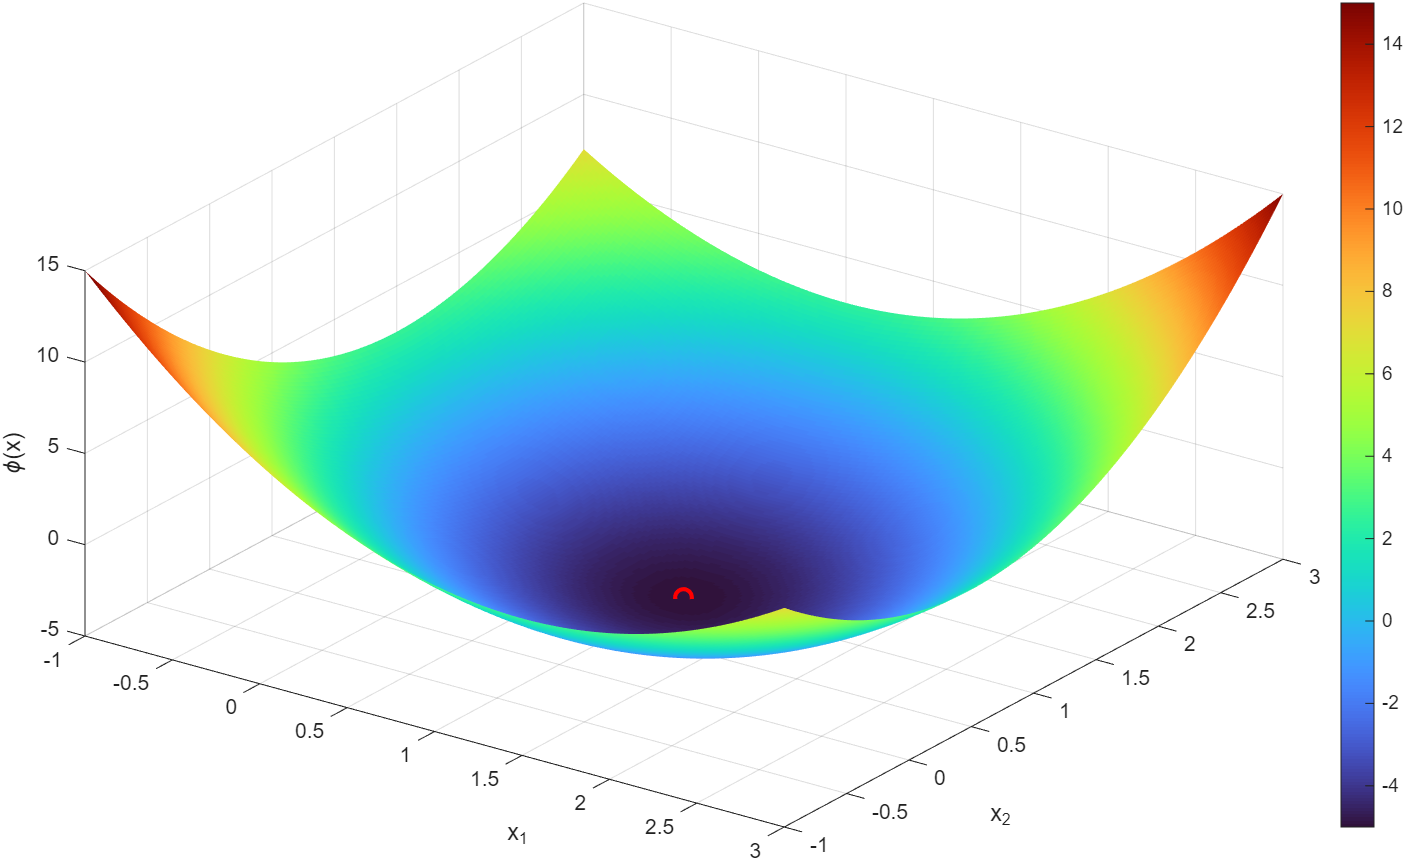
\includegraphics[width=0.6\linewidth]{figs/objective_function.png}
    \caption{This is $\phi$ in 2D. It has a bowl shape. The minimum is circled in red.}
\end{figure}
\end{frame}

%%%%%%%%%%%%%%%%%%%%%%%%%%%%%%%%%%%%%%%%%%%
\begin{frame}{Local Minimum = Absolute Minimum}

\begin{itemize}
    \item Consider a simple 1D example of the $\phi(x) = \frac{1}{2} x^T A x - x^T b,$:
    $$
    \phi(x)=4x^2 - 2x
    $$
        \vfill 
    \item Since $\phi''(x)=8>0$, its critical point is the unique absolute minimum.
        \vfill 
    \item We can find the local minimum calculus:
    \begin{align*}
    \phi'(x) &= 8x-2 \equiv 0\\
            &\implies x =1/4
    \end{align*}

\end{itemize}
\onslide<2>{
        \question{
    How can you find the minimum in higher dimensions?
}
}
\end{frame}

%%%%%%%%%%%%%%%%%%%%%%%%%%%%%%%%%%%%%%%%%%%
\begin{frame}{Gradient of $\phi(x)$}

\begin{itemize}
    \item Since \( x^T b = x_1 b_1 + \cdots + x_n b_n \),  
    \[
    \nabla (x^T b) = [b_1 \quad \cdots \quad  b_n ]^T = b.
    \]
    \item For \( x^T A x \), applying the product rule:
    \[
        \nabla(x^TAx)=(A+A^T)x=2Ax
        \qquad \text{since } A=A^T.
    \]
    \item Therefore the gradient is 
    $$\nabla \phi(x)=\nabla( \frac{1}{2} x^T A x - x^T b) = Ax-b $$
\end{itemize}

\begin{block}{Derivative of $\phi$}
In higher dimensions, the derivative of $\phi(x)$ is 
\[
\nabla \phi(x) = Ax - b.
\]
\end{block}

\end{frame}

%%%%%%%%%%%%%%%%%%%%%%%%%%%%%%%%%%%%%%%%%%%
\begin{frame}{Absolute Minimum of \( \phi(x) \)}

\begin{block}{In 1D}
    \begin{itemize}
        \item Calculate $\phi'(x)$
        \item Set $\phi'(x)=0$
        \item Solve for $x$
    \end{itemize}
\end{block}

\vfill

\begin{block}{In $\mathbb{R}^n$}
    \begin{itemize}
        \item Calculate the gradient:\quad  $\nabla \phi(x) = Ax-b$
        \item Set it equal to zero: \quad\quad$Ax-b=0$
        \item Then solve for $x$: \;\qquad\quad$x = A^{-1}b$
    \end{itemize} 
\end{block}

\vfill 

\question{What do you notice about the minimizer of $\phi(x)$?}


\end{frame}

%%%%%%%%%%%%%%%%%%%%%%%%%%%%%%%%%%%%%%%%%%%
\begin{frame}{Equivalent Problems}
\begin{block}{Problem A}
    Solve the system $Ax=b$ where $A$ is SPD.
\end{block}
\begin{center} 
$\updownarrow$  reformulation
\end{center} \vspace{-2mm}
\begin{block}{Problem B}
    Find the absolute minimum of $\phi(x) = \frac{1}{2} x^T A x - x^T b$ where $A$ is SPD.
\end{block}
\vfill 
\begin{itemize}
    \item Problem B reformulates Problem A as an \textbf{optimization problem}.
    \item \textbf{Gradient methods} can solve problem B. 
\end{itemize}


\keyidea{
For SPD $A$, solving $Ax=b$ is equivalent to minimizing $\phi(x)$.
}

\end{frame}

%%%%%%%%%%%%%%%%%%%%%%%%%%%%%%%%%%%%%%%%%%%

\begin{frame}{Gradient Methods}

{
\define{Gradient Methods}{
Use the gradient to construct successive approximations
to a minimizer of $\phi(x)$.
}
}

\begin{block}{Update}
\[
    x^{(k+1)}
    =
    x^{(k)}
    +
    \alpha_k\;
    s^{(k)}.
\]
\begin{itemize}
    \item $\alpha_k=$ step size 
    \item $s^{(k)}=$ search direction
\end{itemize}
\end{block}

\begin{itemize}
    \item Choose a direction and step size to decrease $\phi$.
    \item For our quadratic, $\nabla\phi(x^{(k)})=-r^{(k)}$.
\end{itemize}

\begin{block}{Stopping Condition}
\[
    \|r^{(k)}\|<\delta.
\]
\end{block}

\end{frame}

%%%%%%%%%%%%%%%%%%%%%%%%%%%%%%%%%%%%%%%%%%%
\begin{frame}{Gradient Descent}

\begin{itemize}
    \item Follow the direction of \textbf{steepest descent}:
    \[
        s^{(k)}
        =-\nabla\phi(x^{(k)})
        =r^{(k)}.
    \]
\end{itemize}

\begin{block}{Gradient Descent Update}
\[
    x^{(k+1)}=x^{(k)}+\alpha r^{(k)},
    \qquad r^{(k)}=b-Ax^{(k)}.
\]
\end{block}

\begin{itemize}
    \item Choose a fixed step size $\alpha>0$.
    \item The step size must be small enough for convergence.
\end{itemize}

\method{Gradient Descent}
{SPD matrix $A$, RHS $b$, step $\alpha$, tolerance}
{Approximate solution to $Ax=b$}
{Move in the direction of steepest descent.}

\end{frame}
%%%%%%%%%%%%%%%%%%%%

\begin{frame}{Gradient Descent}
    \begin{figure}
        \centering
        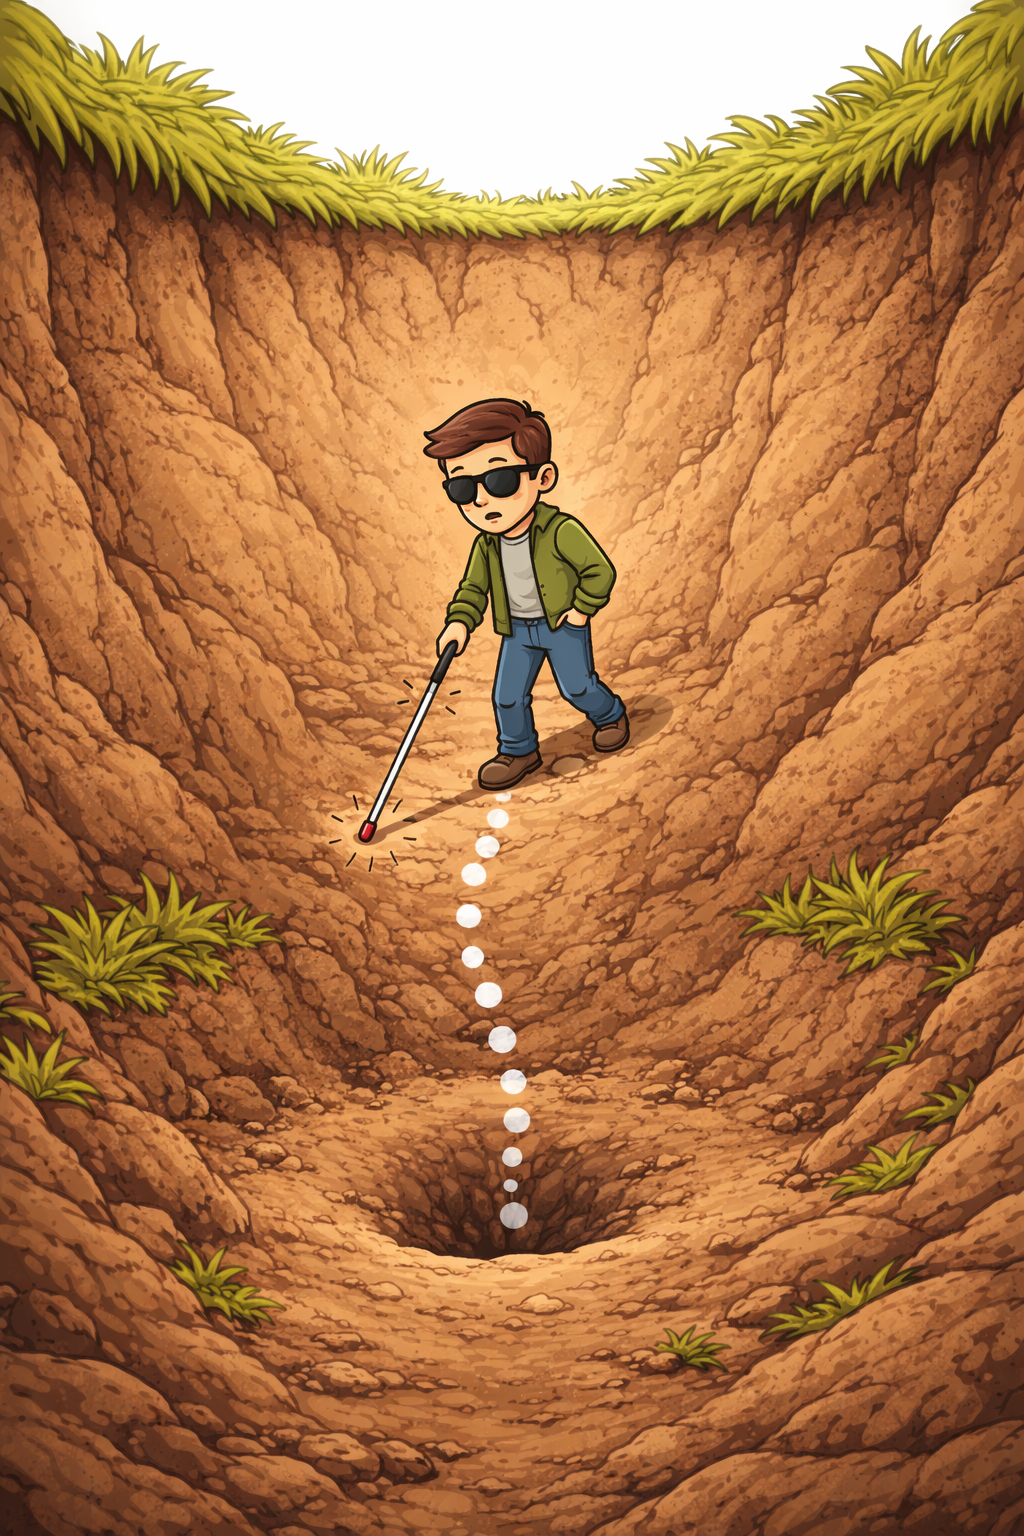
\includegraphics[scale=0.1]{figs/GD_cartoon.png}
    \end{figure}
Gradient descent is like a blind person trying to reach the bottom of a pit.
At each step they feel the slope and move in the steepest downhill direction.
\end{frame}

%%%%%%%%%%%%%%%%%%%%%%%%%%%%%%%%%%%%%%%%%%%

\begin{frame}{Gradient Descent Visualized}
    \begin{center}
        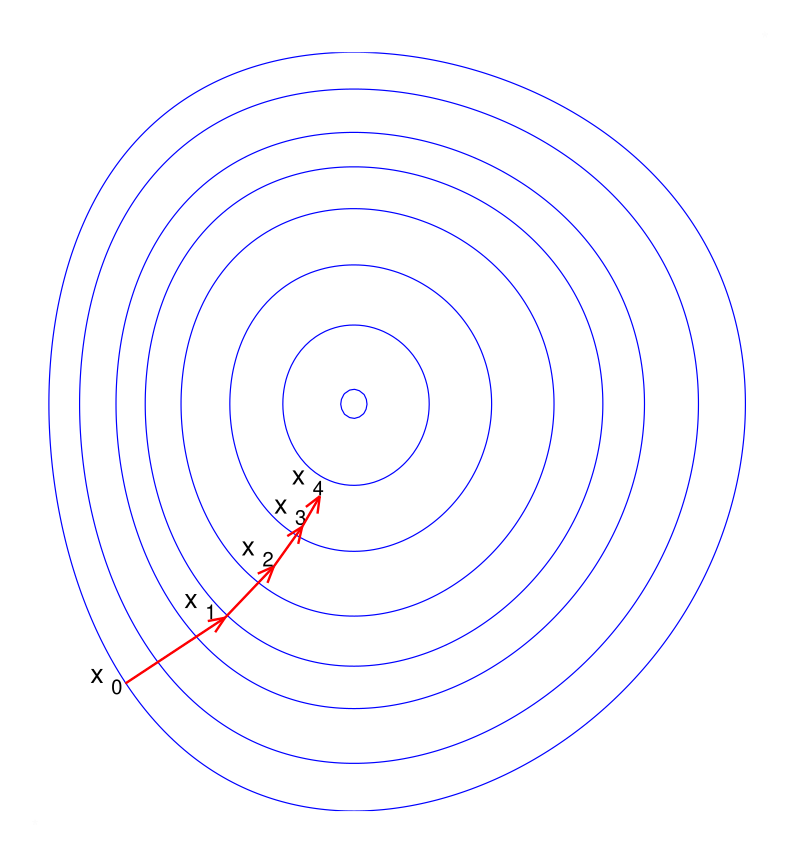
\includegraphics[scale=0.2]{figs/gradient_descent.png}
    \end{center}
    \begin{itemize}
        \item This is a simple example for $2 \times 2$ matrix 
        \item blue curves = contour map for $\phi(x)$
        \item The minimum is at the center of the innermost circle
        \item red arrows = vectors indicating $-\nabla \phi (x_k)$
    \end{itemize}
\end{frame}

%%%%%%%%%%%%%%%%%%%%%%%%%%%%%%%%%%%%%%%%%%%
\begin{frame}[fragile]{Performance}

\cols{

\begin{figure}
    \centering
    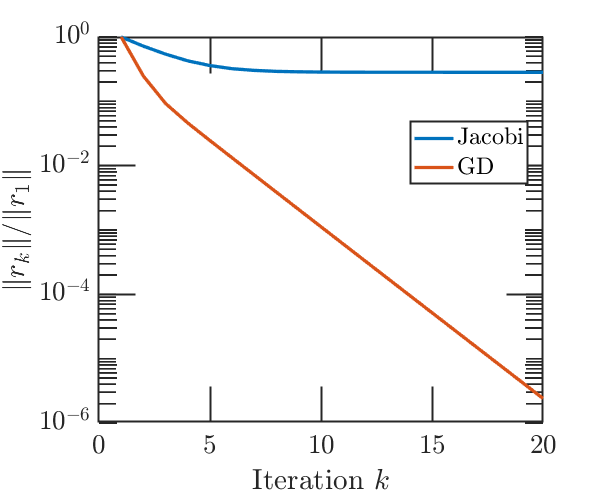
\includegraphics[width=1.0\linewidth]{figs/gd_res.png}
\end{figure}
}{
Pros:
\begin{itemize}
    \item Very easy to code 
    \item One matrix-vector product per iteration.
\end{itemize}
    
}
    \begin{lstlisting}
alpha = 0.8/max(eigs(A));
rnorms = zeros(N,1);
for i = 1:N
    r = b - A*x;         % residue 
    rnorms(i) = norm(r); % compute norm 
    x = x + alpha*r;     % update 
end
    \end{lstlisting}
\end{frame}
%%%%%%%%%%%%%%%%%%%%%%%%%%%%%%%%%%%%%%%%%%%

\begin{frame}{Not the Best Method}

\begin{itemize}
    \item Consider the matrix $$A =  \begin{bmatrix}
        4 & 2\\
        2 & 1.001
    \end{bmatrix}$$

    \item This matrix is SPD, but \texttt{cond(A)=   6.2501e+03}


    \begin{figure}
        \centering
        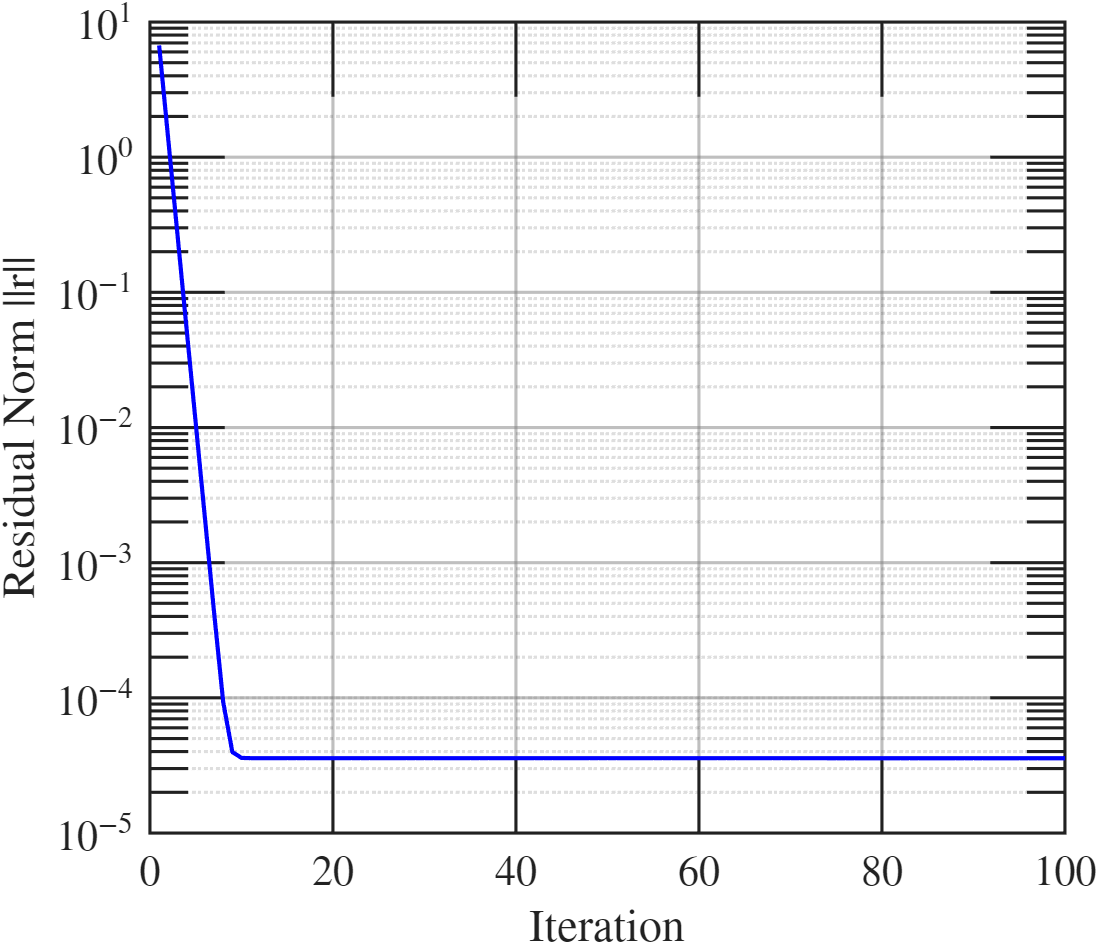
\includegraphics[width=0.4\linewidth]{figs/gd_for_illcond.png}
    \end{figure}
    \item The error cannot achieve machine precision
    
\end{itemize}
    
\end{frame}
%%%%%%%%%%%%%%%%%%%%%%%%%%%%%%%%%%%%%%%%%%%
\begin{frame}{Issues with Gradient Descent}

\begin{itemize}
    \item \textbf{Step size}: too small is slow; too large can diverge.
    \vfill
    \item \textbf{Ill-conditioning}: elongated contours slow progress.
    \vfill
    \item \textbf{Zigzagging}: downhill steps can repeatedly cross the valley.
\end{itemize}

\vfill

\question{
Can we choose a better step size and search direction?
}

\end{frame}


%%%%%%%%%%%%%%%%%%%%%%%%%%%%%%%%%%%%%%%%%%%
\sectionframe{Conjugate Gradient}
%%%%%%%%%%%%%%%%%%%%%%%%%%%%%%%%%%%%%%%%%%%

\begin{frame}{Step Size}
        \begin{itemize}

\item One issue with the Gradient Descent is that $\alpha$ is fixed 

$$ x^{(k+1)} = x^{(k)} + \underbrace{\alpha}_{\footnotesize \text{fixed} } s^{(k)} $$
\vfill 
\item It's suboptimal

\vfill 
\item Annoying to tune

\vfill 
\item It would be better to make $\alpha$ dynamic: 
$$
    \alpha \rightarrow \alpha_k
$$
\vfill 
\end{itemize}
\end{frame}

% ----------

% \begin{frame}{Improving $\alpha$}{Part 1}
% \begin{itemize}

% \begin{block}{Goal}
% Derive a formula for dynamic stepsize $\alpha$ in the gradient descent 
%     \[
%     x^{(k+1)} = x^{(k)} + \alpha_k \, s^{(k)}
%     \]
% where the stepsize is chosen optimally.
% \end{block}

% \item[1.]  Choose $\alpha$ so that $\phi(x^{(k)} + \alpha \,s^{(k)} )$ is minimized
%     \vspace{3mm}
% \item[2.] Use calculus to find critical $\alpha$
%     \begin{align*}    
%     0 &= \frac{d}{d\alpha}\phi(x^{(k)}  + \alpha s^{(k)} )  = \nabla \phi(x^{(k)}  + \alpha s^{(k)} )^T \frac{d}{d\alpha}(x^{(k)}  + \alpha s^{(k)} ) \\ 
%      &= -(r^{(k+1)})^T \frac{d}{d\alpha}(x^{(k)}  + \alpha s^{(k)} ) \\
%      &= -(r^{k+1})^T s^{(k)}.
%     \end{align*}
% \item[3.] We may obtain a formula for the residue 
%     \[
%     r^{(k+1)} = b-Ax^{(k+1)} = b-A(x^{(k)} + \alpha s^{(k)}) = r^{(k)} - \alpha A s^{(k)}
%     \]
% \end{itemize}
% \end{frame}

% %%%%%%%%%%%%%%%%%%%%%%%%%%%%%%%%%%%%%%%%%%%%%%%%%%%%%%%%%%%%%%%%%%%
% \begin{frame}{Improving $\alpha$}{Part 2}
% \begin{itemize}
% \item[4.] Substitute the residue $r^{(k+1)}$, and then solve for $\alpha$
% \begin{align*}
%      0 &= -(r^{(k+1)})^T s^{(k)}\\
%      0 &= -( r^{(k)} - \alpha A s^{(k)})^T s^{(k)}\\
%      (r^{(k)})^T s^{(k)} &= \alpha (s^{(k)})^TA^T  s^{(k)}\\
%      \therefore \alpha &= \frac{(r^{(k)})^T s^{(k)}}{   (s^{(k)})^T A\, s^{(k)}}
% \end{align*}
% \end{itemize}

% \keyidea{
% The dynamic stepsize 
% $$\alpha_k = \frac{(r^{(k)})^T s^{(k)}}{(s^{(k)})^T A\, s^{(k)}}$$
% bypasses the need for tuning and ensures optimal use of each step. 
% }
% \end{frame}

%%%%%%%%%%%%%%%%%%%%%%%%%%%%%%%%%%%%%%%%%%%%%%%%%%%%%%%%%%%%%%%%%%%
\begin{frame}{Improving $\alpha$}{Choosing the Best Step}

\begin{block}{Goal}
Given the search direction $s^{(k)}$, choose the stepsize $\alpha_k$
optimally in
\[
x^{(k+1)} = x^{(k)} + \alpha_k s^{(k)}.
\]
\end{block}

\begin{itemize}

\item[1.] Along the direction $s^{(k)}$, define
\[
g(\alpha)
=
\phi\!\left(x^{(k)}+\alpha s^{(k)}\right).
\]

\item[2.] Choose $\alpha$ to minimize this one-variable function:
\[
\alpha_k = \arg\min_{\alpha} g(\alpha).
\]

\item[3.] Therefore, at the optimal stepsize,
\[
g'(\alpha_k)=0.
\]

\end{itemize}
\end{frame}
%%%%%%%%%%%%%%%%%%%%%%%%%%%%%%%%%%%%%%%%%%%%%%%%%%%%%%%%%%%%%%%%%%%
\begin{frame}{Improving $\alpha$}{The Optimality Condition}
\begin{itemize}
    \item[4.] Using the chain rule,
\begin{align*}
0
&= g'(\alpha) \\[1mm]
&=
\nabla\phi\!\left(x^{(k)}+\alpha s^{(k)}\right)^T
\frac{d}{d\alpha}
\left(x^{(k)}+\alpha s^{(k)}\right) \\[1mm]
&=
\nabla\phi(x^{(k+1)})^T s^{(k)}.
\end{align*}

\item[5.] Recall that the gradient and residual are related
\[
\nabla\phi(x)=Ax-b=-r.
\]

\item[6.] Therefore,
\[
0=-(r^{(k+1)})^T s^{(k)},
\]
or equivalently,
\[
\boxed{(r^{(k+1)})^T s^{(k)}=0.}
\]
\end{itemize}

\keyidea{
At the optimal stepsize, the new residual is orthogonal
to the search direction.
}

\end{frame}
%%%%%%%%%%%%%%%%%%%%%%%%%%%%%%%%%%%%%%%%%%%%%%%%%%%%%%%%%%%%%%%%%%%
\begin{frame}{Improving $\alpha$}{Solving for the Stepsize}

\begin{itemize}
    \item[7.] Rewrite $r^{(k+1})$ in terms of $r^{(k)}$
\begin{align*}
r^{(k+1)}
&= b-Ax^{(k+1)} \\
&= b-A\left(x^{(k)}+\alpha s^{(k)}\right) \\
&= r^{(k)}-\alpha As^{(k)}.
\end{align*}

\item[8.] Substitute this into
\[
(r^{(k+1)})^Ts^{(k)}=0:
\]
and then solve for $\alpha$.

\begin{align*}
0
&=
\left(r^{(k)}-\alpha As^{(k)}\right)^Ts^{(k)} \\[1mm]
&=
(r^{(k)})^Ts^{(k)}
-\alpha(s^{(k)})^TAs^{(k)}.
\end{align*}

Thus,
\[
\boxed{
\alpha_k
=
\frac{(r^{(k)})^Ts^{(k)}}
     {(s^{(k)})^TAs^{(k)}}
}.
\]
\end{itemize}

\end{frame}
%%%%%%%%%%%%%%%%%%%%%%%%%%%%%%%%%%%%%%%%%%%%%%
\begin{frame}{Search Direction}
\begin{itemize}
    \item Gradient Descent with variable step size
    $$
    x^{(k+1)} = x^{(k)} + \alpha_k \, s^{(k)}
    $$
    is still not good enough 
    \vfill 
    \item It cannot prevent zig-zagging 
    \vfill
\end{itemize}

\begin{block}{Goal}
Derive a formula for search direction $s^{(k)}$ in the gradient method 
    \[
    x^{(k+1)} = x^{(k)} + \alpha_k \, s^{(k)}
    \]
which eliminates the zigzagging behavior in GD. 
\end{block}
\end{frame}
%%%%%%%%%%%%%%%%%%%%%%%%%%%%%%%%%%%%%%%%%%%%%%
\begin{frame}{How to improve $s^{(k)}$: Orthogonal Directions}

\begin{itemize}

    \item \textbf{Key Issue:} 
    \begin{itemize}
        \item Redundant search directions
        \item New directions are nearly parallel to old directions  
    \end{itemize}
    \vfill
    \item \textbf{Fix:} Force new directions to be \textit{perpendicular} to previous directions

\end{itemize}
    {
    \define{Orthogonality}{
        \begin{itemize}
        \item Two vectors are \textbf{orthogonal} if \( u^T v = 0 \).
        \item Two vectors are \textbf{A-orthogonal (A-conjugate)} if \( u^T A v = 0 \) where $A$ is $n\times n$.

    \end{itemize}
    }
    }

\end{frame}

%%%%%%%%%%%%%%%%%%%%%%%%%%%%%%%%%%%%%%%%%%%
\begin{frame}{Improving the Search Direction}

\begin{itemize}
    \item Start with the steepest descent direction:
    \[
        s^{(0)}=r^{(0)}.
    \]

    \item At the next iteration, include the previous direction.
\end{itemize}

\begin{block}{New Search Direction}
\[
    s^{(k+1)}=r^{(k+1)}+\beta_k s^{(k)}.
\]
\end{block}

\begin{itemize}
    \item Choose $\beta_k$ so the directions are $A$-conjugate:
    \[
        (\underbrace{s^{(k+1)}}_{\text{new}})^T A \underbrace{s^{(k)}}_{\text{old}}=0.
    \]
\end{itemize}

\end{frame}

%%%%%%%%%%%%%%%%%%%%%%%%%%%%%%%%%%%%%%%%%%%
\begin{frame}{Choosing $\beta_k$}

\begin{itemize}
    \item Substitute the new direction into the conjugacy condition:
    \[
        \bigl(r^{(k+1)}+\beta_k s^{(k)}\bigr)^T
        A s^{(k)}=0.
    \]

    \item Solving for $\beta_k$ gives
    \[
        \beta_k
        =-\frac{(r^{(k+1)})^T A s^{(k)}}
                   {(s^{(k)})^T A s^{(k)}}.
    \]
\end{itemize}

\begin{block}{Simplified Formula for CG}
Using the exact line search and CG orthogonality:
\[
    \beta_k=
    \frac{(r^{(k+1)})^T r^{(k+1)}}
         {(r^{(k)})^T r^{(k)}}.
\]
\end{block}

\keyidea{
Only a scalar correction is needed to update the search direction.
}

\end{frame}

%%%%%%%%%%%%%%%%%%%%%%%%%%%%%%%%%%%%%%%%%%%%%%


%%%%%%%%%%%%%%%%%%%%%%%%%%%%%%%%%%%%%%%%%%%%%%

\begin{frame}{Orthogonal Steps}
\begin{center}
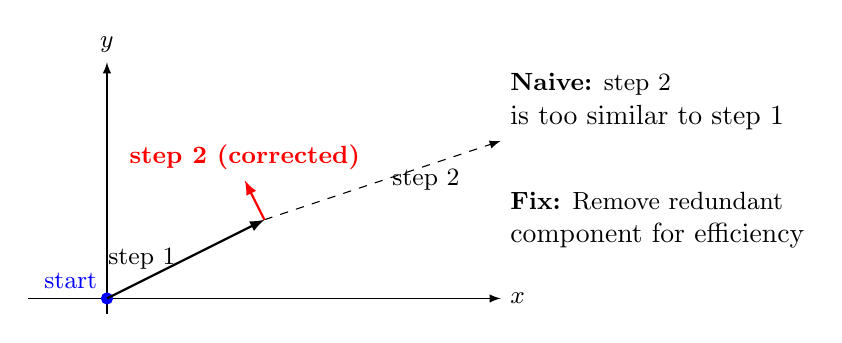
\begin{tikzpicture}[scale=1, >=latex]

    % Axes
    \draw[->] (-1,0) -- (5,0) node[right] {\small $x$};
    \draw[->] (0,-0.2) -- (0,3) node[above] {\small $y$};

    % Initial point
    \filldraw[blue] (0,0) circle (2pt) node[above left] {\small start};

    % First step: right 2, up 1
    \draw[thick, ->] (0,0) -- (2,1) node[midway, left] {\small step 1};

    % Second step (non-orthogonal) right 3, up 1 
    \draw[dashed, ->] (2,1) -- (5,2) node[midway, right] {\small step 2};

    % Orthogonal correction
    \draw[thick, ->, red] (2,1) -- ++(-0.25,0.5) node[above] {\small \textbf{step 2 (corrected)}};

    % % Labels
     \node[align=left, anchor=west] at (5,2.5) {\small \textbf{Naive:} step 2 \\ is too similar to step 1};
     \node[align=left, anchor=west] at (5,1.0) {\small \textbf{Fix:} Remove redundant \\ component for efficiency};

\end{tikzpicture}
\end{center}

\keyidea{
Instead of searching in a near-identical direction, we remove the redundant component to make progress in an independent \textbf{A-orthogonal} direction.
}

\end{frame}


%%%%%%%%%%%%%%%%%%%%%%%%%%%%%%%%%%%%%%%%%%%%%%%

%-------------------------------------------------
\begin{frame}{Other Small Improvements}

\begin{itemize}
\item \textbf{Reuse \(A s^{(k)}\).}  
      The product \(p^{(k)} = A\,s^{(k)}\) is needed  
      \(
        \bigl(s^{(k)}\bigr)^{\!\top}p^{(k)}
      \)
      for \(\alpha_k\) \emph{and} again in the residual update.  
      Compute it \emph{once}, store in a temporary, and the loop needs only \(\operatorname{nnz}(A)\) flops per iteration.

\item \textbf{Short residual recurrence.}
\[
r^{(k+1)} \;=\; r^{(k)} - \alpha_k\,p^{(k)}
\]
      avoids the extra SpMV that
      \(b - A x^{(k+1)}\) would require.

\item \textbf{Dot-product recycling.}  
      The numerator \(r^{(k+1)^{\!\top}}r^{(k+1)}\) is already computed for \(\beta_{k+1}\).  
      Reuse it for the stopping test \(\|r^{(k+1)}\|_2 < \varepsilon\).

\item \textbf{Minimal storage.}  With those tricks, CG needs only four \(n\)-vectors in memory: \(x^{(k)}, r^{(k)}, s^{(k)}, p^{(k)}\).

\end{itemize}

\end{frame}

%%%%%%%%%%%%%%%%%%%%%%%%%%%%%%%%%%%%%%%%%%%%%%%

\begin{frame}[fragile]{Conjugate Gradient}

\begin{lstlisting}[mathescape]
$x_0 = $ initial guess
$r_0 = b-Ax_0$
$s_0 = r_0$
for $k = 0, 1, 2, \dots$
  $\alpha_k = \frac{r_k^T r_k}{s_k^T A s_k}$
  $x_{k+1} = x_k + \alpha_k s_k$
  $r_{k+1} = r_k - \alpha_k A s_k$
  $\beta_{k+1} = r_{k+1}^T r_{k+1} / r_k^T r_k$
  $s_{k+1} = r_{k+1} + \beta_{k+1} s_k$
\end{lstlisting}

\method{Conjugate Gradient}{Given $A$, $b$, tolerance}{Approximation to $Ax=b$}{ Very efficient iterative method
\begin{itemize}
    \item Utilize sparsity of $A$
    \item $\alpha$ is optimized 
    \item $s_k$ are chosen to be A-orthogonal to each other
\end{itemize}
}
\bigskip
\end{frame}
%%%%%%%%%%%%%%%%%%%%%%%%%%%%%%%%%%%%%%%%%%%%%%%%%%%%%%%%%
\begin{frame}{Conjugate Gradient Visualized}

    \cols{
    \begin{center}
        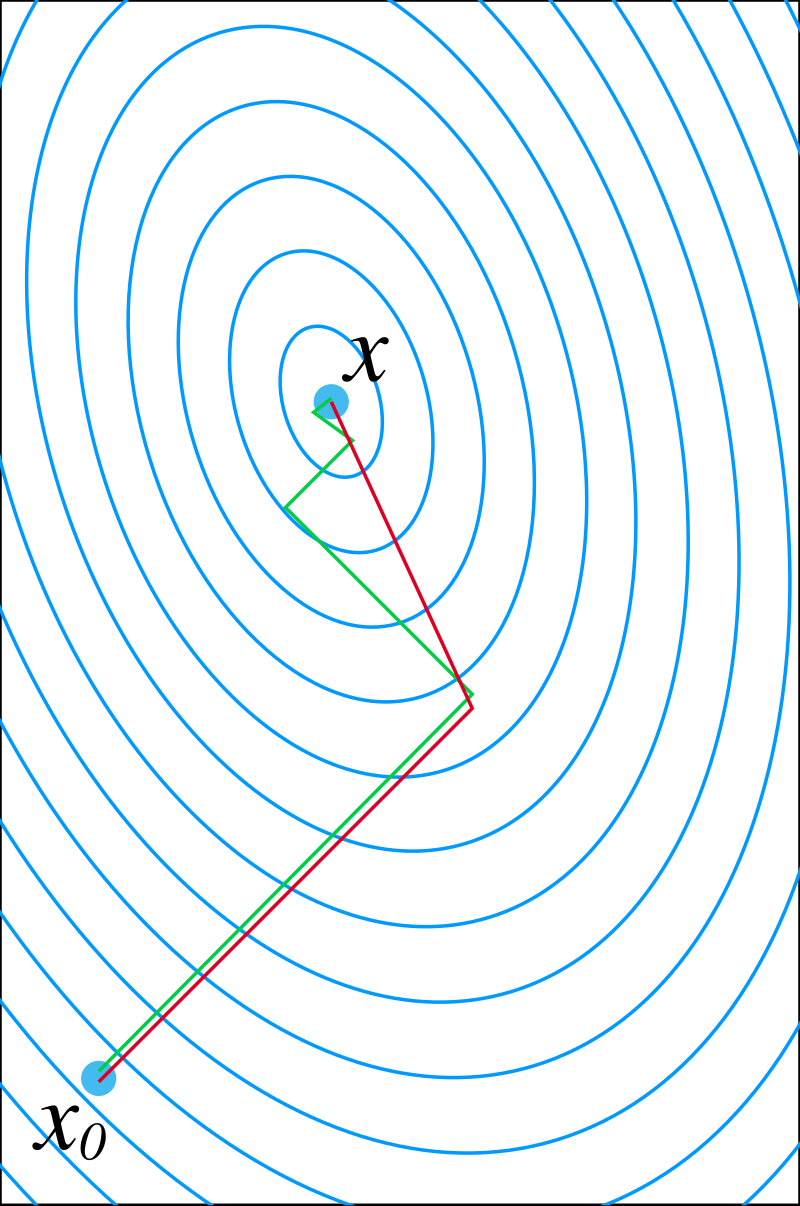
\includegraphics[scale=0.15]{figs/congjugate_gradient.png}
    \end{center}
    }{
    \begin{itemize}
        \item Example $A,\; 2 \times 2$ matrix 
        \item blue curves = contour map
        \item green = gradient descent 
        \item red = conjugate gradient
    \end{itemize}
    \vspace{3mm}
    For a simple $2 \times 2$, CG will converge in just 2 iterations.
    \vspace{3mm}
    }

\end{frame}

%%%%%%%%%%%%%%%%%%%%%%%%%%%%%%%%%%%%%%%%%%%%%%%%%%%%%%%%%
\begin{frame}{Convergence of Conjugate Gradient}

\begin{block}{Exact Arithmetic}
For an $n\times n$ SPD matrix, CG reaches the exact solution
in \textbf{at most $n$ iterations}.
\end{block}

\begin{itemize}
    \item The search directions are mutually $A$-conjugate.
    \vfill
    \item In practice, we stop when $\|r^{(k)}\|<\delta$.
    \vfill
    \item Rounding errors can prevent termination within $n$ iterations.
    \vfill
    \item Often, far fewer than $n$ iterations are needed.
\end{itemize}

\end{frame}

%%%%%%%%%%%%%%%%%%%%%%%%%%%%%%%%%%%%%%%%%%%%%%%%%%%%%%%%%

\begin{frame}{Performance: CG vs. Jacobi}

\cols{
    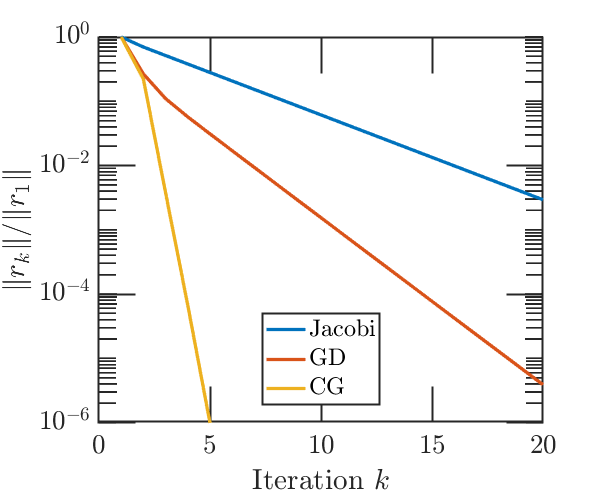
\includegraphics[scale=0.3]{figs/cg_res.png}
}{
\begin{itemize}
    \item The error for Jacobi and CG are shown on a log-linear plot
    \item CG converges much faster than GD
\end{itemize}
}

\keyidea{
\begin{itemize}
    \item CG is a go-to algorithm to solve $Ax=b$ but $A$ must be SPD
    \item CG is better than GD because it uses optimal stepsize and A-orthogonal search directions
\end{itemize}
}
    
\end{frame}


%%%%%%%%%%%%%%%%%%%%%%%%%%%%%%%%%%%%%%%%%%
\end{document}